% +--------------------------------------------------------------------+
% | LaTeX Template                                                     |
% | for K-State Electronic Theses, Dissertations, and Reports          |
% |                                                                    |
% | Comments and guidelines for using the template are shown           |
% | within boxes like this one.                                        |
% |                                                                    |
% | Revised 6/30/06                                                    |
% | 9/14/06: Removed typos                                             |
% | 3/29/13: Commented out hypernat package                            |
% | 4/5/13: Changed to plain bib style
% | 5/17/13: added /cleardoublepage and /phantomsection to
% |          /bibliography to correct TOC page problem
% | 5/17/13: Fixed TOC problem with Dedication, Preface, etc.          |
% +--------------------------------------------------------------------+

% +--------------------------------------------------------------------+
% | Your paper should contain the following sections, except where     |
% | indicated as optional, in the order shown.  Also, all headings     |
% | shown with an asterisk (*) must be centered and in uppercase       |
% | letters:                                                           |
% |                                                                    |
% | Abstract Title Page (doctoral dissertations only)                  |
% | ABSTRACT* (doctoral dissertations only)                            |
% | Title Page                                                         |
% | Copyright Page (Optional - only needed if copyrighting)            |
% | ABSTRACT *                                                         |
% | TABLE OF CONTENTS *                                                |
% | LIST OF FIGURES *                                                  |
% | LIST OF TABLES*                                                    |
% | ACKNOWLEDGMENTS* (Optional)                                        |
% | DEDICATION * (Optional)                                            |
% | PREFACE * (Optional)                                               |
% | Individual Chapters                                                |
% | References and/or bibliography                                     |
% | Appendices (as needed)                                             |
% +--------------------------------------------------------------------+

% +--------------------------------------------------------------------+
% | The LaTex keyword \documentclass selects a particular class to     |
% | associate with the document.  The current documentclass            |
% | {class_diss} generates a Table of Contents that has leading dots   |
% | only on chapter subheadings.  If you prefer a Table of Contents    |
% | that has leading dots for all entries, replace {class_diss}        |
% | with {Mydiss} in the command below.                                |
% |                                                                    |
% +--------------------------------------------------------------------+

\documentclass[final, 12pt,oneside]{class_diss}

% +--------------------------------------------------------------------+
% | The bibliography style is set to a generic superscript. Other      |
% | styles are available in the styles directory.  To use an           |
% | author/year style, you'll need to make several adjustments:        |
% |   1.  In the \bibliographystyle command below, replace "unsrtnat"  |
% |       with the desired style from the \styles directory, e.g.,     |
% |       \bibliographystyle{styles\apa}                               |
% |   2.  In the \bibpunct command (several lines below), change the   |
% |       "s" to an "a"                                                |
% |   3.  Use "\citep" rather than "\cite" when making a citation in   |
% |       the text.                                                    |
% +--------------------------------------------------------------------+

\bibliographystyle{styles\apa}

% +--------------------------------------------------------------------+
% | Now, we add in all external packages that we will use throughout   |
% | the document.  You can add other packages as needed.
% +--------------------------------------------------------------------+

%\usepackage{     caption2} % Customize captions a bit more
\usepackage{      amsmath} % American Mathematics Society standards
%\usepackage{      wrapfig} % Wraps text around a figure or table
\usepackage{     graphicx} % Extended graphics package.
%\usepackage{     fancyhdr} % Efficiently handles headers and footers
%\usepackage{       braket} % Bra-Ket notation package
%\usepackage{     mathrsfs} % Specialized Math fonts (Hamiltonian, etc.)
%\usepackage{boxedminipage} % Boxed text can be produced
%\usepackage{     setspace} % Controls line spacing via \begin{space}

\usepackage{amsxtra}
\usepackage{amssymb}
\usepackage{amsthm}
\usepackage{latexsym}
\usepackage{setspace}

% +--------------------------------------------------------------------+
% | The color package allows one to select colors for hyperlinking     |
% | (see below).                                                       |
% +--------------------------------------------------------------------+

\usepackage[usenames]{color}

% +--------------------------------------------------------------------+
% | Colors defined for use with this template.                         |
% +--------------------------------------------------------------------+

\definecolor{  Pink}{rgb}{1.0, 0.5, 0.5}
\definecolor{Maroon}{rgb}{0.8, 0.0, 0.0}

% +--------------------------------------------------------------------+
% | In the commands below, we use the 'natbib' package, and specify    |
% | the 'sort&compress' option, which condenses                        |
% | citations from (1,2,3,5,9,10,11) to (1-3,5,9-11).  The 'bibpunct'  |
% | option selects various parameters for how the citation will be     |
% | displayed.  In this case, only the comma (separation between       |
% | citations) and the 's' (superscript) arguments are chosen.  The    |
% | other curly braces deal with how to 'wrap' the citation (using     |
% | parentheses, brackets, etc.) and are not needed for the chosen     |
% | style.                                                             |
% +--------------------------------------------------------------------+

\usepackage{natbib}
\bibpunct{}{}{,}{a}{}{}
%\usepackage{hypernat}

% +--------------------------------------------------------------------+
% | Lastly, the hyperref package allows one to hyperlink cross-        |
% | references and figures in a LaTeX document.                        |
% | 3/29/13 - Hypernat package commented out because  it is no longer      |
% | needed with later versions of hyperref and natbib.                 |
% +--------------------------------------------------------------------+

\usepackage[pdftex, plainpages=false, pdfpagelabels]{hyperref}

\hypersetup{
    linktocpage=true,
    colorlinks=true,
    bookmarks=true,
    citecolor=blue,
    urlcolor=red,
    linkcolor=Maroon,
    citebordercolor={1 0 0},
    urlbordercolor={1 0 0},
    linkbordercolor={.7 .8 .8},
    breaklinks=true,
    pdfpagelabels=true,
    }

% +--------------------------------------------------------------------+
% | Page margins are set on 1 inch on all sides.                       |
% +--------------------------------------------------------------------+

\topmargin      = -0.56in
\textheight     =  8.60in
\textwidth      =  6.46in
\oddsidemargin  =  0.02in


% +--------------------------------------------------------------------+
% | The document finally begins here.                                  |
% +--------------------------------------------------------------------+

\doublespacing
\begin{document}

% +--------------------------------------------------------------------+
% | Masters Students -- You Need to Make Some Changes Here

% | The Abstract Title page and Abstract following the Abstract Title
% | page are required only for doctoral dissertations.  For masters
% | theses or reports, comment out or delete the following 7 lines:
% | % +--------------------------------------------------------------------+
% | Abstract Title Page
% |
% |This page is required only for doctoral dissertations.
% +--------------------------------------------------------------------+

% +--------------------------------------------------------------------+
% | This page should not contain a page number.  We use the
% | \thispagestyle[empty] command below to suppress page numbers
% | and other style elements.
% +--------------------------------------------------------------------+

\thispagestyle{empty}

% +--------------------------------------------------------------------+
% | The Abstract Title page begins here                                |
% +--------------------------------------------------------------------+

\pdfbookmark[0]{Title Page}{PDFTitlePage}
%\setcounter{page}{1}

\begin{center}

   \vspace{1cm}

% +--------------------------------------------------------------------+
% | Enter the title of your ETDR below.  Use ALL CAPITAL LETTERS.
% +--------------------------------------------------------------------+

   \large ENTER YOUR TITLE\\

   \vspace{0.5cm}

   by\\

   \vspace{0.5cm}

% +--------------------------------------------------------------------+
% | Enter your name below in ALL CAPITAL LETTERS.
% +--------------------------------------------------------------------+

   \large ENTER YOUR NAME\\

   \vspace{0.5cm}

% +--------------------------------------------------------------------+
% | List previous degrees in mixed case. Include the abbreviation for  |
% | the degree, the name of the university, and the year separated by  |
% | commas. For example:                                               |
% |                                                                    |
% |    B.A., University of Illinois, 2000                              |
% |                                                                    |
% | If desired, it is acceptable to include a city or country with     |
% | the university name. For example:                                  |
% |                                                                    |
% |    B.S., Jillian University, China, 2002                           |
% +--------------------------------------------------------------------+

   Enter Your Previous Degrees\\

   \vspace{0.55cm}
   \rule{2in}{0.5pt}\\
   \vspace{0.75cm}

   {\large AN ABSTRACT OF A DISSERTATION}\\

   \vspace{0.5cm}
   \begin{singlespace}
   submitted in partial fulfillment of the\\
   requirements for the degree\\
   \end{singlespace}

   \vspace{0.5cm}

% +--------------------------------------------------------------------+
% | On the line below, enter the name of your earned degree in ALL
% | CAPITAL LETTERS.  For example: DOCTOR OF PHILOSOPHY
% +--------------------------------------------------------------------+


   {\large ENTER YOUR DEGREE NAME}\\
   \vspace{0.5cm}

% +--------------------------------------------------------------------+
% | On the two lines below, enter the name of your department and the
% | name of the college in mixed case.  For example:
% |
% |     Biochemistry Department
% |     College of Arts and Sciences
% +--------------------------------------------------------------------+

   \begin{singlespace}
   Enter Your Department Name\\
   Enter College Name\\
   \end{singlespace}

   \vspace{0.5cm}

   \begin{singlespace}
   {\Large KANSAS STATE UNIVERSITY}\\
   Manhattan, Kansas\\
   \end{singlespace}

% +--------------------------------------------------------------------+
% | On the line below, enter the year of your graduation.  The year
% | should be the only text on the line.  For example:
% |
% |     2006
% +--------------------------------------------------------------------+

   Enter the year of your graduation\\
   \vspace{1cm}

\end{center}
 through \end{abstract}.  You will also
% | need to uncomment two lines under "Abstract" below.
% |
% +--------------------------------------------------------------------+

%% +--------------------------------------------------------------------+
% | Abstract Title Page
% |
% |This page is required only for doctoral dissertations.
% +--------------------------------------------------------------------+

% +--------------------------------------------------------------------+
% | This page should not contain a page number.  We use the
% | \thispagestyle[empty] command below to suppress page numbers
% | and other style elements.
% +--------------------------------------------------------------------+

\thispagestyle{empty}

% +--------------------------------------------------------------------+
% | The Abstract Title page begins here                                |
% +--------------------------------------------------------------------+

\pdfbookmark[0]{Title Page}{PDFTitlePage}
%\setcounter{page}{1}

\begin{center}

   \vspace{1cm}

% +--------------------------------------------------------------------+
% | Enter the title of your ETDR below.  Use ALL CAPITAL LETTERS.
% +--------------------------------------------------------------------+

   \large ENTER YOUR TITLE\\

   \vspace{0.5cm}

   by\\

   \vspace{0.5cm}

% +--------------------------------------------------------------------+
% | Enter your name below in ALL CAPITAL LETTERS.
% +--------------------------------------------------------------------+

   \large ENTER YOUR NAME\\

   \vspace{0.5cm}

% +--------------------------------------------------------------------+
% | List previous degrees in mixed case. Include the abbreviation for  |
% | the degree, the name of the university, and the year separated by  |
% | commas. For example:                                               |
% |                                                                    |
% |    B.A., University of Illinois, 2000                              |
% |                                                                    |
% | If desired, it is acceptable to include a city or country with     |
% | the university name. For example:                                  |
% |                                                                    |
% |    B.S., Jillian University, China, 2002                           |
% +--------------------------------------------------------------------+

   Enter Your Previous Degrees\\

   \vspace{0.55cm}
   \rule{2in}{0.5pt}\\
   \vspace{0.75cm}

   {\large AN ABSTRACT OF A DISSERTATION}\\

   \vspace{0.5cm}
   \begin{singlespace}
   submitted in partial fulfillment of the\\
   requirements for the degree\\
   \end{singlespace}

   \vspace{0.5cm}

% +--------------------------------------------------------------------+
% | On the line below, enter the name of your earned degree in ALL
% | CAPITAL LETTERS.  For example: DOCTOR OF PHILOSOPHY
% +--------------------------------------------------------------------+


   {\large ENTER YOUR DEGREE NAME}\\
   \vspace{0.5cm}

% +--------------------------------------------------------------------+
% | On the two lines below, enter the name of your department and the
% | name of the college in mixed case.  For example:
% |
% |     Biochemistry Department
% |     College of Arts and Sciences
% +--------------------------------------------------------------------+

   \begin{singlespace}
   Enter Your Department Name\\
   Enter College Name\\
   \end{singlespace}

   \vspace{0.5cm}

   \begin{singlespace}
   {\Large KANSAS STATE UNIVERSITY}\\
   Manhattan, Kansas\\
   \end{singlespace}

% +--------------------------------------------------------------------+
% | On the line below, enter the year of your graduation.  The year
% | should be the only text on the line.  For example:
% |
% |     2006
% +--------------------------------------------------------------------+

   Enter the year of your graduation\\
   \vspace{1cm}

\end{center}

%
%\begin{abstract}
%   \setcounter{page}{-1}
%   \pdfbookmark[0]{Abstract}{PDFAbstractPage}
%   %!TEX root = etdrtemplate.tex
% +--------------------------------------------------------------------+
% | Abstract Page
% +--------------------------------------------------------------------+

\pagestyle{empty}
%\vspace{1cm}
\setlength{\baselineskip}{0.8cm}

\indent

% +--------------------------------------------------------------------+
% | Enter the text of your abstract below, maximum of 350 words.
% +--------------------------------------------------------------------+

The future of Medical Devices is their interoperability. Nowadays, medical devices works rather independently, which cause accidents we could avoid if different devices would communicate. Dr. Julian Goldman developed idea of "Integrated Clinical Environment" (ICE). It is series of standards, which describes medical device interoperability. SAnToS lab created Medical Device Coordination Framework (MDCF), which is prototype implementation of ICE idea.

AADL (Architecture Analysis \& Design Language) is modeling language for representing hardware and software. It is used for real-time, safety critical and embedded systems. AADL allows for the description of both software and hardware parts of a system. It is used to describe architecture, but AADL allows to add behavioral extensions through annex languages. BLESS (Behavior Language for Embedded Systems with Software) is AADL annex sub language defining behavior of components. The goal of BLESS is automatically-checked correctness proofs of AADL models of embedded electronic systems with software.

Ada is one of the most popular (along with C/C++) programming language targeted at embedded and real-time systems. SPARK Ada is subset of Ada, designed for the development of safety and security critical systems. It contains subset, which allows to reason about and prove correctness of program and its entities.

Nowadays, there is a trend to generate code from models. The ultimate goal of research, which this thesis if part of, is to create AADL/BLESS to SPARK Ada translator. Ultimately set of standardized AADL/BLESS models for medical devices would be created. From these models SPARK Ada code base would be generated. It would be further extended by developers.

This thesis propose mapping from AADL/BLESS to SPARK Ada. As an example of Medical Device, PCA (Patient Controlled Analgesia) pump is used. The foundation for this work is "Integrated Clinical Environment Patient-Controlled Analgesia Infusion Pump System Requirements" document \cite{PcaReq} and AADL Models with BLESS annexes created by Brian Larson. In addition to proposed mapping, PCA pump prototype was created. As a platform for prototyping, BeagleBoard-xM device was used. Some components of PCA pump prototype are verified by SPARK tools and Bakar Kiasan.

%   \vfill
%\end{abstract}

% +--------------------------------------------------------------------+
% | Title Page -- Required for both Doctoral and Masters Students
% +--------------------------------------------------------------------+

% +--------------------------------------------------------------------+
% | Title Page
% +--------------------------------------------------------------------+

\newpage

% +--------------------------------------------------------------------+
% | This page should not contain a page number.  We use the
% | \thispagestyle[empty] command below to suppress page numbers
% | and other style elements.
% +--------------------------------------------------------------------+

\thispagestyle{empty}

% +--------------------------------------------------------------------+
% | The Title page begins here.
% +--------------------------------------------------------------------+

\begin{center}

   \vspace{1cm}

% +--------------------------------------------------------------------+
% | On the line below, replace "ENTER YOUR TITLE" with the title of
% | your ETDR.  Use all CAPITAL LETTERS.
% +--------------------------------------------------------------------+

   %\large VERIFICATION OF HIGH-INTEGRITY SYSTEMS IN SPARK/ADA PROGRAMS BY EXAMPLE OF PCA-PUMP\\
   \large MODEL DRIVEN DEVELOPMENT FOR MEDICAL DEVICES IN AADL/BLESS AND SPARK/ADA: PCA PUMP PROTOTYPE\\

   \vspace{0.3cm}

   by\\

   \vspace{0.3cm}

% +--------------------------------------------------------------------+
% | On the line below, replace "ENTER YOUR NAME" with your name.  Use
% | mixed case, for example, Laura Bush.
% +--------------------------------------------------------------------+

   \large Jakub Jedryszek\\

   \vspace{0.3cm}

% +--------------------------------------------------------------------+
% | On the line below, replace List"Enter Your Previous Degrees"
% | with your previous degrees in mixed case. Include the abbreviation
% | for the degree, the name of the university, and the year
% | separated by commas. For example:                                  |
% |                                                                    |
% |    B.A., University of Illinois, 2000                              |
% |                                                                    |
% | If desired, it is acceptable to include a city or country with     |
% | the university name. For example:                                  |
% |                                                                    |
% |    B.S., Jillian University, China, 2002                           |
% +--------------------------------------------------------------------+

   B.S., Wroclaw University of Technology, Poland, 2012\\
   B.A., Wroclaw University of Economics, Poland, 2012\\

   \vspace{0.35cm}
   \rule{2in}{0.5pt}\\
   \vspace{0.65cm}

   {\large A THESIS}\\

   \vspace{0.3cm}
   \begin{singlespace}
   submitted in partial fulfillment of the\\
   requirements for the degree\\
   \end{singlespace}

   \vspace{0.3cm}

% +--------------------------------------------------------------------+
% | On the line below, replace "ENTER YOUR DEGREE NAME" with the name
% | of your earned degree in ALL CAPITAL LETTERS.
% +--------------------------------------------------------------------+

   {\large MASTER OF SCIENCE}\\
   \vspace{0.3cm}

% +--------------------------------------------------------------------+
% | On the two lines below, replace "Enter Your Department Name" and
% | "Enter Your College Name" with the name of your department and the
% | name of the college in mixed case.  For example:
% |
% |     Biochemistry Department
% |     College of Arts and Sciences
% +--------------------------------------------------------------------+

   \begin{singlespace}
   Department of Computing and Information Sciences\\
   College of Engineering\\
   \end{singlespace}

   \vspace{0.3cm}

   \begin{singlespace}
   {\large KANSAS STATE UNIVERSITY}\\
   Manhattan, Kansas\\
   \end{singlespace}

% +--------------------------------------------------------------------+
% | On the line below, replace "Graduation Year" with the year of
% | your graduation.  The year should be the only text on the line.
% | For example:
% |
% |     2013
% +--------------------------------------------------------------------+

   2014\\
   \vspace{0.3cm}

    \end{center}

    \begin{flushright}
    Approved by:\\
    \vspace{0.3cm}
    \begin{singlespace}
    Major Professor


% +--------------------------------------------------------------------+
% | On the line below, replace "Enter Your Major Professor's Name"
% | with  the name of your major professor in mixed case.  Use the
% | format Firstname Lastname.  For example:
% |
% |     Lori Goetsch
% |
% +--------------------------------------------------------------------+

    John Hatcliff\\
    \end{singlespace}
    \end{flushright}

% +--------------------------------------------------------------------+
% | If you have co-major professors, comment out the lines above from
% | \begin{flushright} through \end{flushright} and uncomment the lines
% | below.
% +--------------------------------------------------------------------+

%\begin{flushright}
%   Approved by:\\
%  \vspace{ 0.3cm}
%   \begin{singlespace}
%   Co-Major Professor\\
%   Enter Your Co-Major Professor's Name\\
%   \vspace{.25cm}
%   Co-Major Professor\\
%   Enter Your Co-Major Professor's Name\\
%   \end{singlespace}
%\end{flushright}


% +--------------------------------------------------------------------+
% | Copyright Page -- Required for both Doctoral and Masters Students
% +--------------------------------------------------------------------+

% +--------------------------------------------------------------------+
% | Copyright Page
% +--------------------------------------------------------------------+

\newpage

\thispagestyle{empty}

\vspace*{1.5cm}

\begin{center}

{\bf \Huge Copyright}

\vspace{1cm}

% +--------------------------------------------------------------------+
% | On the line below, replace "Enter Your Name" with your name
% | Use the same form of your name as it appears on your title page.
% | Use mixed case, for example, Lori Goetsch.
% +--------------------------------------------------------------------+

   \Large Jakub Jedryszek\\

   \vspace{0.5cm}

% +--------------------------------------------------------------------+
% | On the line below, replace "Graduation Year" with the year of your
% | graduation, for example,
% |
% |     2013
% |
% +--------------------------------------------------------------------+

   2014\\

   \vspace{0.5cm}

\end{center}


% +--------------------------------------------------------------------+
% |  Abstract -- Required for both Doctoral and Masters Students
% +--------------------------------------------------------------------+

\begin{abstract}

% +--------------------------------------------------------------------+
% | For masters theses or reports, uncomment the following commands:
% +--------------------------------------------------------------------+

   \setcounter{page}{-1}
   \pdfbookmark[0]{Abstract}{PDFAbstractPage}

    %!TEX root = etdrtemplate.tex
% +--------------------------------------------------------------------+
% | Abstract Page
% +--------------------------------------------------------------------+

\pagestyle{empty}
%\vspace{1cm}
\setlength{\baselineskip}{0.8cm}

\indent

% +--------------------------------------------------------------------+
% | Enter the text of your abstract below, maximum of 350 words.
% +--------------------------------------------------------------------+

The future of Medical Devices is their interoperability. Nowadays, medical devices works rather independently, which cause accidents we could avoid if different devices would communicate. Dr. Julian Goldman developed idea of "Integrated Clinical Environment" (ICE). It is series of standards, which describes medical device interoperability. SAnToS lab created Medical Device Coordination Framework (MDCF), which is prototype implementation of ICE idea.

AADL (Architecture Analysis \& Design Language) is modeling language for representing hardware and software. It is used for real-time, safety critical and embedded systems. AADL allows for the description of both software and hardware parts of a system. It is used to describe architecture, but AADL allows to add behavioral extensions through annex languages. BLESS (Behavior Language for Embedded Systems with Software) is AADL annex sub language defining behavior of components. The goal of BLESS is automatically-checked correctness proofs of AADL models of embedded electronic systems with software.

Ada is one of the most popular (along with C/C++) programming language targeted at embedded and real-time systems. SPARK Ada is subset of Ada, designed for the development of safety and security critical systems. It contains subset, which allows to reason about and prove correctness of program and its entities.

Nowadays, there is a trend to generate code from models. The ultimate goal of research, which this thesis if part of, is to create AADL/BLESS to SPARK Ada translator. Ultimately set of standardized AADL/BLESS models for medical devices would be created. From these models SPARK Ada code base would be generated. It would be further extended by developers.

This thesis propose mapping from AADL/BLESS to SPARK Ada. As an example of Medical Device, PCA (Patient Controlled Analgesia) pump is used. The foundation for this work is "Integrated Clinical Environment Patient-Controlled Analgesia Infusion Pump System Requirements" document \cite{PcaReq} and AADL Models with BLESS annexes created by Brian Larson. In addition to proposed mapping, PCA pump prototype was created. As a platform for prototyping, BeagleBoard-xM device was used. Some components of PCA pump prototype are verified by SPARK tools and Bakar Kiasan.

    \vfill

\end{abstract}

% +--------------------------------------------------------------------+
% | We use the following code to suppress page numbers and other
% | style issues we do not want present on a given page.               |
% +--------------------------------------------------------------------+

%\thispagestyle{empty} Looks like it's ok to remove this line
\newpage
\pagenumbering{roman}

% +--------------------------------------------------------------------+
% | On the line below, set the number to represent the page number of
% | the Table of Contents page.  For example, if the Table of Contents
% | page is the 8th page of your document, enter 8 in the brackets.  This
% | number may vary, depending on the length of your abstract.
% |
% | Numbers do not appear on the title and abstract pages, but they are
% | included in the page count.  The Table of Contents page is the
% | first page on which page numbers are displayed.
% +--------------------------------------------------------------------+

\setcounter{page}{8}

% +--------------------------------------------------------------------+
% | Here, we will generate our Table of Contents (TOC) entries.        |
% | This adds the section to the TOC and then generates the indicated  |
% | section.                                                           |
% +--------------------------------------------------------------------+

\phantomsection
\addcontentsline{toc}{chapter}{Table of Contents}

\tableofcontents
\listoffigures
\listoftables

%\hfill  Are these lines necessary?
%\hfill

% +--------------------------------------------------------------------+
% | Acknowledgements Page
% |
% | If you choose not to have an Acknowledgements page, comment out
% | or delete the following 3 lines.
% +--------------------------------------------------------------------+

\phantomsection
\addcontentsline{toc}{chapter}{Acknowledgements}
%!TEX root = JakubJedryszek2014.tex
% +--------------------------------------------------------------------+
% | Acknowledgements Page (Optional)                                   |
% +--------------------------------------------------------------------+

\newpage
\vspace*{0.9cm}
\begin{center}
{\bf \Huge Acknowledgments}
\end{center}

\setlength{\baselineskip}{0.8cm}

%\pdfbookmark[0]{Acknowledgements}{PDF_Acknowledgements}
\phantomsection
\addcontentsline{toc}{chapter}{Acknowledgements}

\setlength\epigraphwidth{1.0\textwidth}
\setlength\epigraphrule{0pt}
\makeatletter
\patchcmd{\epigraph}{\@epitext{#1}}{\itshape\@epitext{#1}}{}{}
\makeatother

\epigraph{"Showing gratitude is one of the simplest yet most powerful things humans can do for each other."}{--- \textup{Randy Pausch}, Last Lecture}


I would like to say thank you to all people, who helped me pursue Master of Science program in Computer Science at Kansas State University. Many thanks to Dr. Andrew Rys who encourage me to apply for Graduate School, and was always helpful with an advice. I wish to thank, my major professor, Dr. John Hatcliff who admitted me to SAnToS Laboratory research group, and enabled me to be involved in research. I met there many passionate people and great researchers. Furthermore, without Dr. Hatcliff's guidance, this thesis will not be accomplished. Thanks to Dr. Robby, who was always helping me in my research, giving valuable suggestions and ideas. Thank you to Jason Belt for sharing his knowledge and experience with me, which played significant role in my research career. Thanks to Brian Larson, whose work, was inspiration of my Master thesis. Many thanks to Dr. Eugene Vasserman for serving on my committee and for his valuable suggestions about this work. A special thanks for Venkatesh Prasad Ranganath. Conversations with him and his suggestions played significant role in accomplishing this thesis.


% +--------------------------------------------------------------------+
% | Dedication Page
% |
% | If you choose not to have a Dedication page, comment out
% | or delete the following 3 lines.
% +--------------------------------------------------------------------+

\phantomsection
\addcontentsline{toc}{chapter}{Dedication}
% +--------------------------------------------------------------------+
% | Dedication Page (Optional)
% +--------------------------------------------------------------------+

\newpage
\vspace*{0.9cm}
\begin{center}
{\bf \Huge Dedication}
\end{center}

\setlength{\baselineskip}{0.8cm}

%\pdfbookmark[0]{Dedication}{PDF_Dedication}

% +--------------------------------------------------------------------+
% | Enter the text for your dedication in the space below this box.
% +--------------------------------------------------------------------+

This template uses a separate file for each section of your ETDR:
title page, abstract, preface, chapters, reference, etc.  This
makes it easier to organize and work with a lengthy document.  The
template is configured with page margins required by the Graduate
School and will automatically create a table of contents, lists of
tables and figures, and PDF bookmarks.

Although the template gives you a foundation for creating your
ETDR, you will need a working knowledge of LaTeX in order to
produce a final document.  You should be familiar with LaTeX
commands for formatting text, equations, tables, and other
elements you will need to include in your ETDR.

This template uses a separate file for each section of your ETDR:
title page, abstract, preface, chapters, reference, etc.  This
makes it easier to organize and work with a lengthy document.  The
template is configured with page margins required by the Graduate
School and will automatically create a table of contents, lists of
tables and figures, and PDF bookmarks.

Although the template gives you a foundation for creating your
ETDR, you will need a working knowledge of LaTeX in order to
produce a final document.  You should be familiar with LaTeX
commands for formatting text, equations, tables, and other
elements you will need to include in your ETDR.

This template uses a separate file for each section of your ETDR:
title page, abstract, preface, chapters, reference, etc.  This
makes it easier to organize and work with a lengthy document.  The
template is configured with page margins required by the Graduate
School and will automatically create a table of contents, lists of
tables and figures, and PDF bookmarks.

Although the template gives you a foundation for creating your
ETDR, you will need a working knowledge of LaTeX in order to
produce a final document.  You should be familiar with LaTeX
commands for formatting text, equations, tables, and other
elements you will need to include in your ETDR.


% +--------------------------------------------------------------------+
% | Preface Page
% +--------------------------------------------------------------------+

\addcontentsline{toc}{chapter}{Preface}
% +--------------------------------------------------------------------+
% | Preface (Optional)
% +--------------------------------------------------------------------+

\newpage
\vspace*{0.9cm}
\begin{center}
{\bf \Huge Preface}
\end{center}

\setlength{\baselineskip}{0.8cm}

%\pdfbookmark[0]{Preface}{PDF_Preface}

% +--------------------------------------------------------------------+
% | Enter text of your Preface in the space below this box.
% +--------------------------------------------------------------------+

This template uses a separate file for each section of your ETDR:
title page, abstract, preface, chapters, reference, etc.  This
makes it easier to organize and work with a lengthy document.  The
template is configured with page margins required by the Graduate
School and will automatically create a table of contents, lists of
tables and figures, and PDF bookmarks.

Although the template gives you a foundation for creating your
ETDR, you will need a working knowledge of LaTeX in order to
produce a final document.  You should be familiar with LaTeX
commands for formatting text, equations, tables, and other
elements you will need to include in your ETDR.

This template uses a separate file for each section of your ETDR:
title page, abstract, preface, chapters, reference, etc.  This
makes it easier to organize and work with a lengthy document.  The
template is configured with page margins required by the Graduate
School and will automatically create a table of contents, lists of
tables and figures, and PDF bookmarks.

Although the template gives you a foundation for creating your
ETDR, you will need a working knowledge of LaTeX in order to
produce a final document.  You should be familiar with LaTeX
commands for formatting text, equations, tables, and other
elements you will need to include in your ETDR.

This template uses a separate file for each section of your ETDR:
title page, abstract, preface, chapters, reference, etc.  This
makes it easier to organize and work with a lengthy document.  The
template is configured with page margins required by the Graduate
School and will automatically create a table of contents, lists of
tables and figures, and PDF bookmarks.

Although the template gives you a foundation for creating your
ETDR, you will need a working knowledge of LaTeX in order to
produce a final document.  You should be familiar with LaTeX
commands for formatting text, equations, tables, and other
elements you will need to include in your ETDR.


\phantomsection
% +--------------------------------------------------------------------+
% | We use arabic (1, 2, 3...) page numbering starting from page 1.    |
% | Note, however, that there are many pages where this is not the     |
% | desired behavior - such as the Title page, or abstract.  In these  |
% | cases, we can use \thispagestyle{empty} to suppress page numbers,  |
% | and other general style issues that we've defined globally.        |
% +--------------------------------------------------------------------+

\newpage
\pagenumbering{arabic}
\setcounter{page}{1}

% +--------------------------------------------------------------------+
% | Here is where we include individual sections of the thesis or
% | dissertation.                                                      |
% +--------------------------------------------------------------------+

% +--------------------------------------------------------------------+
% | Chapters
% +--------------------------------------------------------------------+

% +--------------------------------------------------------------------+
% | Sample Chapter
% |
% | This file provides examples of how to
% | - insert a figure with a caption
% | - construct a table with a caption
% | - create subsections within the chapter
% | - insert a reference to a Figure or Table
% | - make a citation
% +--------------------------------------------------------------------+

\cleardoublepage

% +--------------------------------------------------------------------+
% | Replace "Chapter Title" below with the title of your chapter.  LaTeX
% | will automatically number the chapters.
% +--------------------------------------------------------------------+

\chapter{Chapter Title}
\label{makereference1}

In this chapter, there will be examples of various features you
may want to incorporate into your document. Here's an example of a
figure inserted into the text:

\begin{figure}[htb]%t=top, b=bottom, h=here

    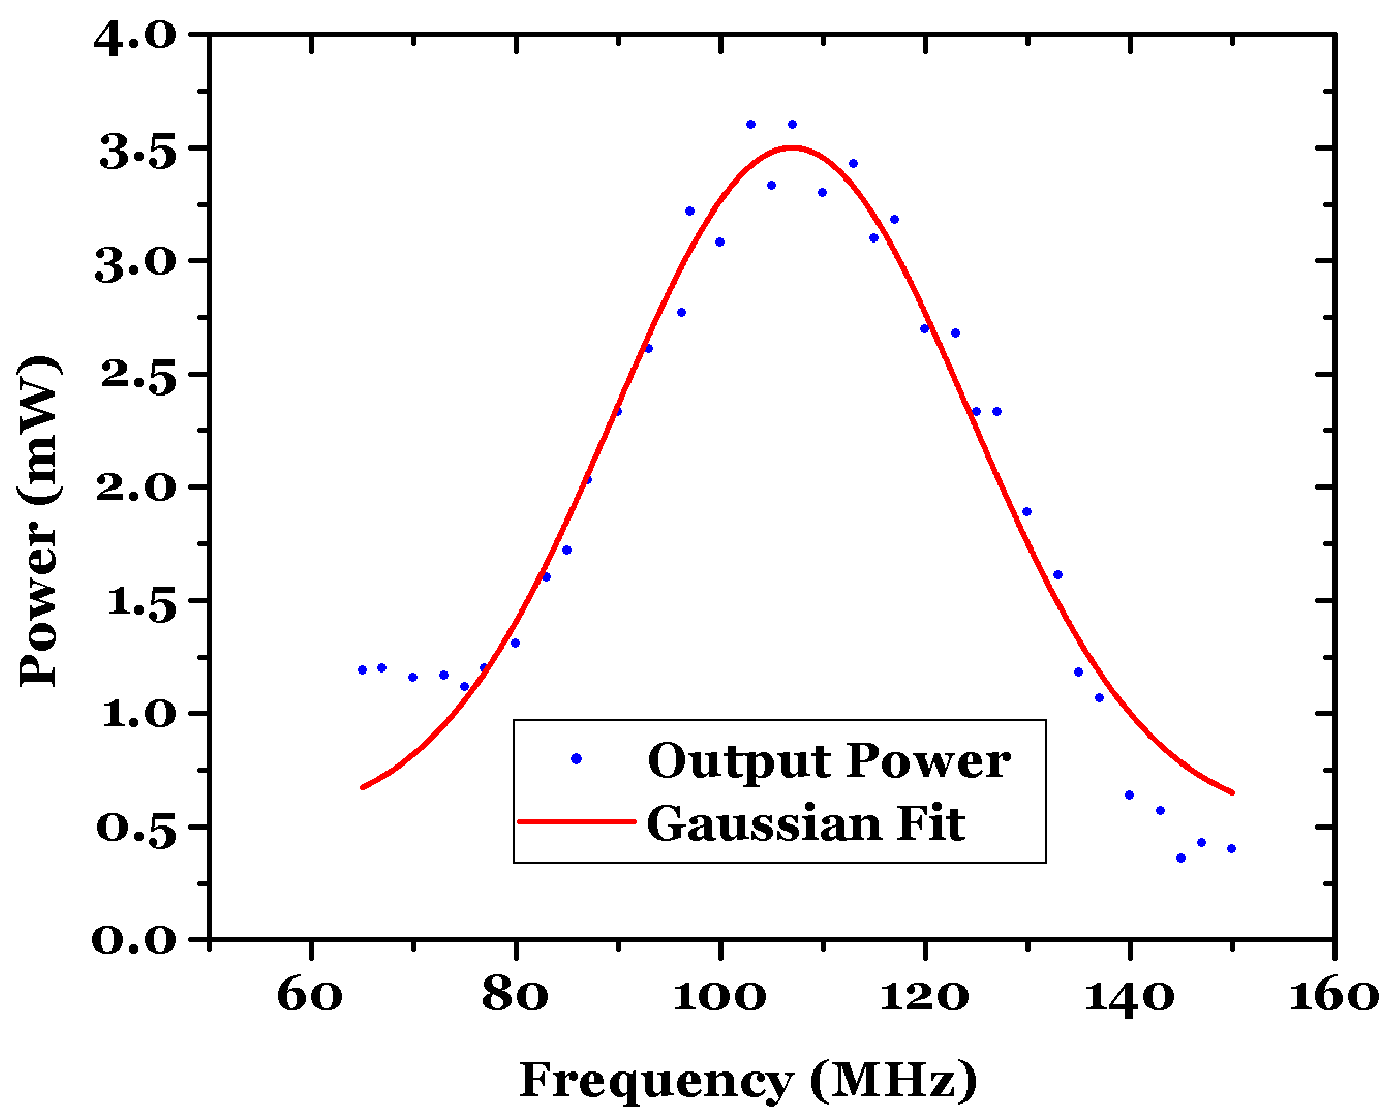
\includegraphics[height=2.5in]{figures/graph.png}

    \caption[Optional: Short caption to appear in List of
    Figures]{Full caption to appear below the Figure}

    \label{figure1}
\end{figure}

% +--------------------------------------------------------------------+
% |To create cross-references to figures, tables and segments
% |of text, LaTeX provides the following commands:
% |   \label{marker}
% |   \ref{marker}
% |   \pageref{marker}
% | where {marker} is a unique identifier.
% |
% | In the line above, we use \label{figure1} to mark a location
% | we wish to refer to later.  LATEX replaces \ref by the number of
% | the chapter, section, subsection, figure, or table after which the
% | corresponding \label command was issued. \pageref prints the page
% | number of the page where the \label command occurred.
% |
% +--------------------------------------------------------------------+

Here is an example of a Table:

\begin{table}

% +--------------------------------------------------------------------+
% | We include the command \begin{center} to center the table
% | horizontally on the page.  Note use of the command \end{center}
% | to turn off centering after the table is defined.
% +--------------------------------------------------------------------+
    \begin{center}

% +--------------------------------------------------------------------+
% | The table is created with this command
% |
% | \begin{tabular}[pos]{table spec}
% |
% | The "pos" argument specifies the vertical position of the table relative to
% | the baseline of the surrounding text.  Use t, b, or c to specify alignment
% | at the top, bottom, or center.
% |
% | The "table spec" command defines the format of the table
% |   l for a column of left-aligned text
% |   r for a column of right-aligned text
% |   c for centered text
% |   p{width} for a column containing justified text with line breaks
% |   | for a vertical line
% +--------------------------------------------------------------------+

    \begin{tabular}[c]{|c|c|c|}
        \hline
        Column 1 Heading & Column 2 Heading & Column 3 Heading \\
        \hline
        Col 1 Row 1 & Col 2 Row 1 & Col 3 Row 1\\
        Col 1 Row 2 & Col 2 Row 2 & Col 3 Row 2\\
        Col 1 Row 3 & Col 2 Row 3 & Col 3 Row 3\\
        \hline
    \end{tabular}
    \caption{Caption to appear below the table}
    \label{table1}
   \end{center}
\end{table}

% +--------------------------------------------------------------------+
% | Replace \section headings below with the title of your
% | subsections.  LaTeX will automatically number the subsections 1.1,
% | 1.2, 1.3, etc.
% +--------------------------------------------------------------------+

\section{Making References to Figures or Tables}
\label{makereference1.1}

In this paragraph, we want to refer to Fig.~\ref{figure1}
mentioned at the beginning of this chapter.  We also refer to the
Table~\ref{table1}.

\section{Making a Reference to a Chapter Subsection}
\label{makereference1.2}

In this section, we refer back to text mentioned in
Section~\ref{makereference1.1} on page~\pageref{makereference1.1}.

\section{Making a Citation}
\label{makereference1.3}

Here's an example of a citation to a single
work.~\cite{CT:Weiner:1999} It's also possible to make multiple
citations.~\cite{CT:Phillips:1985, ARP:Loy:1974}


% +--------------------------------------------------------------------+
% | Uncomment the lines below to add additional chapters.  Name the
% | files chapter2.tex for Chapter 2, chapter3.tex for Chapter 3, etc.
% +--------------------------------------------------------------------+

% +--------------------------------------------------------------------+
% | Sample Chapter 2
% +--------------------------------------------------------------------+

\cleardoublepage

% +--------------------------------------------------------------------+
% | Replace "This is Chapter 2" below with the title of your chapter.
% | LaTeX will automatically number the chapters.
% +--------------------------------------------------------------------+

\chapter{This is Chapter 2}
\label{makereference2}

In this chapter, I want to refer to Chapter~\ref{makereference1}, so
I'm going to use the slash ref command along with the
"makereference" label which I assigned back at the beginning of
Chapter 1.

\section{Page Number References}
\label{makereference2.1} I should also be able to refer to a
specific page number, such as page~\pageref{makereference1}.  Of
course, I'll need to have a slash label command and a unique name in
each section that I want to be able to refer to later in the text.

\section{Referring to Sections Within Chapter 1}
\label{makereference2.2} Now, I'm going to refer to different
sections within Chapter 1. I gave an example of a figure in
section~\ref{makereference1.1} and an example of a table in
section~\ref{makereference1.2}.  In
section~\ref{makereference1.3}, we looked at examples of
bibliographic citations.

% +--------------------------------------------------------------------+
% | Sample Chapter 3
% +--------------------------------------------------------------------+

\cleardoublepage

% +--------------------------------------------------------------------+
% | Replace "This is Chapter 3" below with the title of your chapter.
% | LaTeX will automatically number the chapters.
% +--------------------------------------------------------------------+

\chapter{This is Chapter 3}
\label{makereference3}

Here are more examples of referring to previous sections.  In
Chapter~\ref{makereference} there were several sections, including
section~\ref{makereference1.1}, section~\ref{makereference1.2},
and section~\ref{makereference1.3}.

Likewise, in Chapter~\ref{makereference2}, there are
sections~\ref{makereference2.1} and ~\ref{makereference2.2}.

%\input{chapter4.tex}
%\input{chapter5.tex}

% +-------------------------------------------------------------------------+
% | References                                                              |
% +-------------------------------------------------------------------------+

% +-------------------------------------------------------------------------+
% | In order for WinEDT to index references correctly, it has to know where |
% | the file resides.  The following command is prefaced by %, and will be  |
% | ignored completely by LaTeX.  However, WinEDT will use this line to     |
% | access the external .bib bibliography file.  Also note that WinEDT can  |
% | read file path names with either "\" or "/" - LaTeX, however, doesn't   |
% | like "\", so it's easier to store a path name in the "Unix" style.      |
% +-------------------------------------------------------------------------+

%Included for Gather Purpose only.  Do NOT uncomment:
%input "references.bib"

% +--------------------------------------------------------------------+
% | This template uses the BibTeX program to format references.  The
% | lines below create a separate Bibliography section and add
% | an entry for "Bibliography" to the Table of Contents.  The actual
% | data for your references (author, title, journal, date, etc.) are
% | entered in the references.bib file.  See that file for information
% | on how to enter references.
% +--------------------------------------------------------------------+

\cleardoublepage
\phantomsection
\addcontentsline{toc}{chapter}{Bibliography}
\bibdata{references}
\bibliography{references}

% +--------------------------------------------------------------------+
% | Finally, we generate the appendix.  To add or delete appendices,
% | add or remove the line
% |
% |     \input{appendixX.tex}
% |
% | where "X" is the letter designation of the Appendix (A, B, C, etc.)
% | You should have one \input{appendixX.tex} line and a corresponding
% | file appendixX.tex for each appendix.                                 |
% +--------------------------------------------------------------------+

\appendix
%!TEX root = etdrtemplate.tex
% +--------------------------------------------------------------------+
% | Appendix A Page (Optional)                                         |
% +--------------------------------------------------------------------+

\cleardoublepage

\chapter{Title for This Appendix}
\label{Appendix:Key1}

Content of this appendix.


% +--------------------------------------------------------------------+
% | Enter text for your Appendix page in the space below this box.     |
% |                                                                    |
% +--------------------------------------------------------------------+

% +--------------------------------------------------------------------+
% | Appendix B Page (Optional)                                         |
% +--------------------------------------------------------------------+

\cleardoublepage

\chapter{PCA Pump Prototype - translated from AADL/BLESS}
\label{Appendix:PPP_Trahslated}

%code listings with numbers


\end{document}
